\chapter*{Лекция 2 (2023-09-13). Виды сходимости случайных величин. Предельные теоремы
теории вероятностей. Закон больших чисел}

Пусть на $(\Omega, \mathscr A, \mathsf P)$ задана случайная величина $\xi$ и
последовательность случайных величин $\xi_1, \xi_2, \dots$. Поскольку случайная
величина есть \textsl{функция} от элементарных исходов, имеет смысл говорить о
разных видах сходимости. Рассмотрим их.

\section{Сходимость почти наверное}

\begin{definition}\label{def:pn}
	Говорят, что последовательность случайных величин $ \{\xi_n\} $ \emph{сходится почти
	наверное} к случайной величине $ \xi $ и пишут $\xi_n \toPN \xi$, если
	\[
		P\left(\lim_{n\to\infty} \xi_n = \xi \right) = 1.
	\]
\end{definition}

\begin{ex}
  Пусть $\Omega = [0, 1]$, $\mathscr A$ --- $\sigma$-алгебра измеримых
	подмножеств, $\mathsf P(A) = \operatorname{mes} A$.

	Определим
	\[
	  \xi_n(\omega) = \begin{cases} 1, &0\leqslant \omega < 1/n,\\
	  0, &\text{иначе}. 
    \end{cases}
	\]
  Тогда
	\[
		\forall \omega \neq 0\quad \xi_n(\omega) \to 0,
	\]
	то есть
	\[
		P\left(\lim_{n\to\infty} \xi_n=0\right) = 1.
	\]
\end{ex}

\begin{dfnbis}{def:pn}
	\label{def:pnbis}
	Говорят, что последовательность случайных величин $ \{\xi_n\} $ \emph{сходится почти
	наверное} к случайной величине $ \xi $ и пишут $\xi_n \toPN \xi$, если для
	сколь угодно малого $ \varepsilon > 0 $ выполняется
	\[
		\lim_{n\to\infty} \mathsf P\left\{ \omega\colon \sup\limits_{m\geqslant n}
		|\xi_n-\xi| > \varepsilon \right\} = 0.
	\]
\end{dfnbis}

\begin{utv}
	Определения {\rm\ref{def:pn}} и {\rm\ref{def:pnbis}} эквивалентны.
\begin{proof}
  Первое утверждение эквивалентно следующему:
  \[
  		\mathsf P \left( \xi_n \not\to \xi \right) = 0.
  \]
 
	По оперделению пердела 
	\[
		(\xi_n \to \xi) = \bigcap_{r=1}^\infty \bigcup_{n=1}^\infty\bigcap_{m\geqslant n}
		\left( |\xi_m - \xi| \leqslant 1/r \right),
	\]
а значит, 
\[
	(\xi_n \not\to \xi) = \bigcup_{r=1}^\infty \bigcap_{n=1}^\infty \bigcup_{m\geqslant n}
	\left( |\xi_m - \xi| > 1/r \right).
\]
В нашем случае будем иметь 
\[
	P\left(\bigcup_{r=1}^\infty \bigcap_{n=1}^\infty \bigcup_{m\geqslant n} (|\xi_m -
	\xi| \leqslant 1/r)\right),
\]
то есть для всех $ r \geqslant 1 $ получим
\[
	P\left(\bigcap_{n=1}^\infty \bigcup_{m\geqslant n} \left( |\xi_m - \xi| > 1/r
	\right)\right) = 0.
\]

Обозначим
\[
	B_n := \left\{\sup_{m\geqslant n} |\xi_m - \xi| > 1/r\right\} =
\left\{\bigcup_{m\geqslant n} (|\xi_m - \xi| > 1/r)\right\}.
\]
Тогда для всех $ k $ $ B_{k+1}
\subset B_k $ и $ \bigcap_{n=1}^\infty B_n = \varnothing $. По теореме о
непрерывности вероятности 
\[
	\lim_{n\to\infty} P(B_n) =  
	\lim_{n\to\infty} P \left(\sup_{m\geqslant n} |\xi_m - \xi| > 1/r \right) = 0.
\]

\end{proof}
\end{utv}



\section{Сходимость по вероятности}
\begin{definition}
	Говорят, что последовательность случайных величин $ \{\xi_n \}$ \emph{сходится
	по вероятности} и пишут $\xi_n \toP \xi$, если
	\[
		\forall \varepsilon > 0 \quad \lim_{n\to\infty}
		\mathsf P\left\{\omega \colon|\xi_n-\xi|>\varepsilon\right\} = 0.
	\]
\end{definition}

\begin{theorem}
  Если последовательность случайных величин почти наверное сходится к случайной
	величине $ \xi $, то эта же последовательность будет сходиться к ней по
	вероятности:
	\[
		\xi_n \toPN \xi \Rightarrow \xi_n \toP \xi.
	\]
\end{theorem}

\begin{proof}
  Очевидно. %TODO: (proof)
\end{proof}

%\begin{remark*}
%  Обратное, вообще говоря, не верно.
%\end{remark*}
\begin{ex} Обратное, вообще говоря, неверно. Действительно, пусть $ \Omega = [0,
	1]$, $ \mathscr A $ --- $ \sigma $-алгебра измеримых подмножеств, $ \mathsf
	P(A) = \operatorname{mes} A $. Для $ 2^k \leqslant n < 2^{k+1} $ определим
	последовательность 
	\[
		\xi_n(\omega) = \begin{cases}
			1, & \frac{n-2^k}{2^k} < \omega < \frac{n+1-2^k}{2^k},\\
			0, & \text{иначе}.
		\end{cases}
	\]
Для любого $ \varepsilon \in (0, 1) $ в этом случае имеем 
\[
	P(|\xi_n| > \varepsilon ) = \frac{1}{2^k} \to 0 \quad \text{при } n\to\infty,
\]
при этом $ \xi_n(\omega) \not\to 0 $ ($ \mathsf P $-п. н.).	
\end{ex}

\begin{theorem}
  Если последовательность $\{ \xi_n \}$ монотонно убывает (возрастает) и $\xi_n \toP \xi$, то
	\[
		\xi_n \toPN \xi.
	\]
\end{theorem}
\begin{proof}
Пусть $ \{\xi_n\} $ монотонно убывает и $ \xi_n \toP 0 $ (в случае возрастания
рассматривается последовательность $ \{\xi_n - \xi\} $). Тогда 
\[
	\left( \sup_{m\geqslant n}|\xi_m - \xi| > \varepsilon \right) = \left(
	\sup_{m\geqslant n} |\xi_m| > \varepsilon \right) = \left( \sup_{m\geqslant}
\xi_m > \varepsilon \right) = (\xi_n > \varepsilon). 
\]

\end{proof}

\begin{theorem}
  Если $\xi_n \toP \xi$, то из последовательности $\{ \xi_n \}$ можно выбрать
	подпоследовательность $\{ \xi_{n_k} \}$ такую, что
	\[
		\xi_{n_k} \toPN \xi.
	\]
\end{theorem}
\begin{proof}
  Без доказательства. %TODO: (proof)
\end{proof}

\section{Сходимость по распределению (слабая)}

\begin{definition}\label{def:d}
  Говорят, что последовательность \emph{сходится по распределению} и пишут $\xi_n \toD \xi$ или $F_{\xi_n} (x) \Rightarrow F_\xi (x)$, если для любой непрерывной ограниченной функции $g(x)$ выполняется:
  \[
		\lim_{n\to\infty}\int\limits_{-\infty}^{+\infty} g(x) \,
		dF_{\xi_n}(x) =
		\int\limits_{-\infty}^{+\infty} g(x) \, dF_\xi(x),
\]
или, что то же самое, 
\[
	\lim_{n\to\infty} \mathsf M g(\xi_n) = \mathsf M g(\xi).
\]
\end{definition}

\begin{dfnbis}{def:d}
	\label{def:dbis}
  $F_{\xi_n} (x) \Rightarrow F_\xi(x)$, если $F_{\xi_n}(x) \to F_\xi(x)$ в
	каждой точке непрерывности $F_\xi(x)$. Значит,
\[
	P(\xi_n < x) \xrightarrow[]{n\to\infty} P(\xi<x).
\]
\end{dfnbis}

\begin{theorem}
	Определения {\rm \ref{def:d}} и {\rm \ref{def:dbis}} эквивалентны.
\end{theorem}
\begin{proof} 
	Без доказательства. %TODO: (proof)
\end{proof}



\section{Сходимость в среднем порядка r}
\begin{definition}
	Будем говорить, что последовательность случайных величин \emph{сходится в
	среднем порядка $ r $} к случайной величине $ \xi $ и писать $ \xi_n \toR \xi
	$, если  
	\[
	\lim_{n\to\infty}\mathsf M |\xi_n - \xi|^r = 0.
	\]
	
\end{definition}

\begin{utv}
	Сходимость к $ \xi $ в среднем порядка $ r $ влечёт
	\[
		\xi_n\toR\xi \implies \xi_n \toP \xi
	\]
	сходимость к $ \xi $ по вероятности.
\end{utv}
\begin{proof}
	Применим неравенство Чебышёва и получим 
	\[
			P_\xi(|\xi_n - \xi| \geqslant x) = P (|\xi_n - \xi|^r \geqslant x^r )
			\leqslant \frac{\mathsf M |\xi_n - \xi|^r}{x^r}.
	\]
\end{proof}

\begin{ex}[факультативно]
	Пусть $ \{\xi_n\} $ --- последовательность независимых случайных величин,
	распределённых по закону
	\begin{table}[h!]
		\centering
	\begin{tabular}{|c|c|c|}
		\hline
		$ \xi_n , x_n $ &0 &1 \\\hline
		$ P_\xi(\xi_n = x_n) $ & $ 1 - 1/n $ & $ 1/n $\\\hline
	\end{tabular}.
\end{table}

Тогда  
\[
		P(|\xi_n| > \varepsilon) = P(\xi_n = 1) = \frac{1}{n} \to 0,
\]
а значит, 
\[
		\xi_n \toP 0.
\]
С другой стороны
\begin{multline*}
	P(\xi_n \to 0) = P(|\xi_m| < \varepsilon, \forall m \geqslant n) \leqslant \\
	\leqslant P(|\xi_m| < \varepsilon, \forall n \leqslant m < N) = \prod_{m=0}^N
	P(\xi_m = 0) = \\
	= \frac{n-1}{n}\frac{n}{n+1}\ldots
	\frac{N-1}{N} = \frac{n-1}{N} \to 0
\end{multline*}
при $ N \to \infty $.
\end{ex}


\section{Предельные теоремы}
\begin{theorem}[неравенства Чебышёва]
Для любого $ x > 0 $ имеют место неравенства 
\[
		P(|\xi|\geqslant x) \leqslant \frac{\mathsf M |\xi|}{x}, \qquad
		P(|\xi-\mathsf M\xi|\geqslant x) \leqslant \frac{\mathsf D\xi}{x^2}.
\]
\end{theorem}
\begin{proof}
	\begin{gather*}
		|\xi| = |\xi|\cdot I_{(|xi| \geqslant x)} + |\xi| \cdot I_{(|\xi|<x)}
		\geqslant |\xi| \cdot I_{(|\xi|\geqslant x)} \geqslant x \cdot I_{(|\xi|
		\geqslant x)},\\
		\mathsf M|\xi| \geqslant \mathsf M \left[ x\cdot I_{(|\xi|\geqslant x)}
		\right] = x \mathsf M \left[ I_{(|\xi| \geqslant x)} \right]  = x P(|\xi|
		\geqslant x).
\end{proof}

\begin{corollary} 
\[
		P(|\xi-\mathsf M\xi|< x) \geqslant 1 - \frac{\mathsf D\xi}{x^2}.
\]
\end{corollary}

\begin{theorem}[закон больших чисел Чебышёва]
	Пусть $ \{\xi_n\} $ --- независимые случайные величины и существует
	такая константа $ c > 0 $, что все $\mathsf D \xi_i \leqslant c$,
	$i=\overline{1,2,\ldots, n}$. Тогда при любом $ \varepsilon > 0 $  
	\[
		\lim_{N\to\infty} P_\xi \left( \left| \frac{\xi_1 + \xi_2 + \ldots +
		\xi_N}{N} - \frac{\mathsf M \xi_1 + \mathsf M\xi_2 + \ldots + \mathsf
	M\xi_N}{n} \right| < \varepsilon \right) = 1.
	\]
\end{theorem}
\begin{proof}
  Пусть  
  \[
  		\zeta_N = \frac{\xi_1 + \xi_2 + \ldots + \xi_N}{N}.
  \]
  Тогда
	\begin{align*}
		\mathsf M \zeta_N &= \frac{1}{N}\sum_{k=1}^N \mathsf M\xi_k,\\
		\mathsf D\zeta_N &= \frac{1}{N^2}\sum_{k=1}^N \mathsf D \xi_k \leqslant
		\frac{c}{N}.
\end{proof}
Следовательно, 
\[
		P(|\zeta_N - \mathsf M\zeta_N| < x) \geqslant 1 - \frac{c}{x^2N} \to 1
\]
при $ N \to \infty $. Здесь используется сходимость по вероятности 
\[
	\frac{1}{N}\sum_{k=1}^N \xi_k -\frac{1}{N} \sum_{k=1}^N \mathsf M\xi_k \toP 0.
\]



\begin{theorem}[центральная предельная теорема]
	Если случайные величины $ \{\xi_n\} $ независимы, одинаково распределены и
	имеют конечные $ \mathsf M\xi_i = a $, $ \mathsf D\xi_i = \sigma^2 > 0 $, то 
	\[
		\lim_{n\to\infty} P_\xi \left( \frac{\xi_1 + \xi_2 + \ldots + \xi_n -
		na}{\sigma \sqrt n} < x \right)  = \Phi(x),
	\]
	где используется сходимость по распределению.

\begin{theorem}[Ляпунов]
Пусть случайные величины $ \xi_1, \xi_2, \ldots $ --- независимы, имеют конечные
моменты $ \mathsf M \xi_k = a_k $, $ \mathsf D\xi_k = b^2_k $, $ \mathsf
M|\xi_k-a_k|^3 = c^3_k $. Обозначим $ A_n = \sum^n_{k=1} a_k $, $ B^2_n =
\sum^n_{k=1} b^2_k $, $ C^3_n = \sum^n_{k=1}c^3_k $, причём $ c_n/B_n \to 0 $.
Тогда 
\[
	\lim_{n\to\infty} P \left( \frac{\xi_1+\xi_2+\ldots+\xi_n-A_n}{B_n} < x
		\right) = \Phi(x),
\]
где используется сходимость по распределению 
\[
		\frac{\xi_1+\xi_2+\ldots+\xi_n-A_n}{B_n} \toD \mathscr N(0,1).
\]

\begin{theorem}[Хинчин] 
	Пусть $ \xi_1,\xi_2,\ldots $ --- одинаково распределеннные случайные величины
	с конечным математическим ожиданием $ a $.

	Тогда при любом $ \varepsilon > 0 $ имеем  
	\[
		\lim_{N\to\infty} P \left( \left| \frac{\xi_1+\xi_2+\ldots+\xi_N}{N} - a
		\right| < \varepsilon \right)  = 1,
	\]
	где используется сходимость по вероятности  
	\[
			\frac{\xi_1+\xi_2+\ldots+\xi_N}{N} \toP a.
	\]

\begin{theorem}[Марков]
	Пусть $ \xi_1,\xi_2,\ldots $ --- последовательность случайных величин,
	удовлетворяющая условию  
	\[
		\lim_{n\to\infty} \frac{1}{n^2} \mathsf D [\sum_{k=1}^n \xi_k] = 0.
	\]
	Тогда при сколь угодно малом $ \varepsilon > 0 $ имеем 
	\[
		\lim_{N\to\infty} P \left( \left| \frac{\xi_1 + \xi_2 + \ldots + \xi_N}{N} -
		\frac{\mathsf M \xi_1 + \mathsf M\xi_2 + \ldots + \mathsf M \xi_N}{N}\right|
	< \varepsilon \right) = 1,
	\]
где используется сходимость по вероятности  
\[
		\frac{\xi_1 + \xi_2 + \ldots + \xi_n}{N} - \frac{\mathsf M\xi_1 + \mathsf
		M\xi_2 + \ldots + \mathsf M\xi_N}{N} \toP 0.
\]	
\end{theorem}

\begin{theorem}[необходимое и достаточное условие]
	Пусть $\{\xi_n\}$ --- последовательность случайных величин с $ \mathsf M\xi_k
	= a_k$. Тогда закон больших чисел имеет место тогда и только тогда, когда  
	\[
			\lim_{N\to\infty} P \left( \left| \frac{\xi_1 + \xi_2 + \ldots + \xi_N}{N} -
		\frac{\mathsf M \xi_1 + \mathsf M\xi_2 + \ldots + \mathsf M \xi_N}{N}\right|
	< \varepsilon \right) = 1,
	\]
где используется сходимость по вероятности  
\[
		\frac{\xi_1 + \xi_2 + \ldots + \xi_N}{N} - \frac{\mathsf M \xi_1 + \mathsf
		M\xi_2 + \ldots + \mathsf \xi_N}{N} \toP 0.
\]
	

\begin{theorem}[усиленный закон больших чисел Колмогорова]
	Пусть $ \xi_1, \xi_2, \ldots $ --- независимые и одинаково распределение
	случайные величины. Для того чтобы  
	\[
			\frac{\xi_1 + \xi_2 + \ldots _ \xi_n}{n} \toPN a,
	\]
	необходимо и достаточно, чтобы существовало конечное
	\[
		\mathsf M\xi_n = a,
	\]
	где используется сходимость почти наверное: 
	\[
			\frac{\xi_1+\xi_2+\ldots+\xi-n}{n} \toPN a.
	\]
	


\section{Резюме}
\begin{figure}[h!]
	\centering
	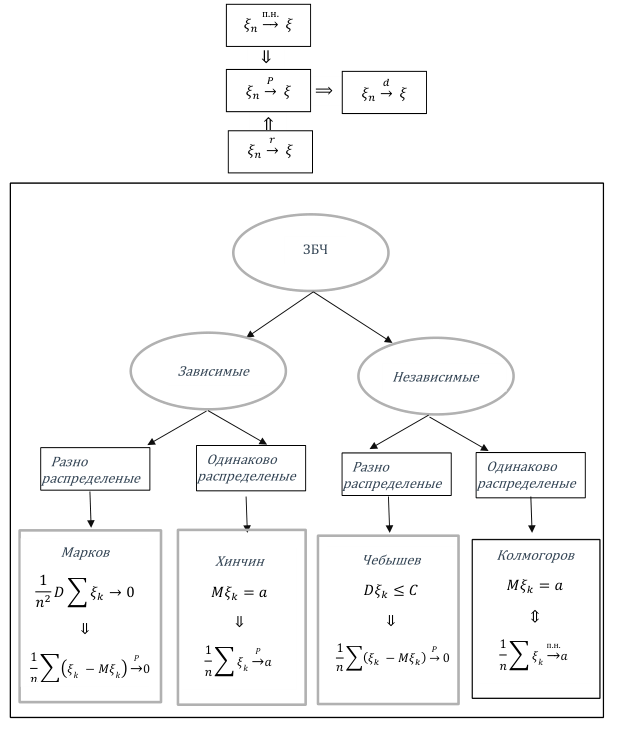
\includegraphics[width=0.8\textwidth]{Figures/resume.png}
	\label{fig:resume}
\end{figure}
